\documentclass[12pt,letterpaper,times]{article}%book, beamer
%Inicia preámbulo

%\include{tesis}


%\usepackage{fourier}
\usepackage{mathpazo}
\usepackage{antpolt}

% to change the fonts

\usepackage{array}

\usepackage{pdfpages}
\usepackage[utf8]{inputenc}
%\usepackage[numbers]{natbib}
\usepackage[english]{babel}
\usepackage{mathptmx}
\usepackage{amsmath}
\usepackage{graphicx}

\usepackage{xcolor}

%\usepackage[margin=1.5cm]{geometry}
\usepackage{fancyhdr}
\usepackage{parskip}
\usepackage[colorlinks=false]{hyperref}
\usepackage{amsmath}
\usepackage{amsmath,amsfonts}
\usepackage{amssymb}
\usepackage{mathrsfs}
\usepackage{siunitx}
%\usepackage[usenames]{color}
\usepackage{multirow} % para las tablas
%\usepackage[spanish,es-tabla]{babel}
\usepackage{hieroglf}
\usepackage{caption}
\usepackage{subcaption}
\usepackage{wrapfig}
\usepackage{booktabs}
%\usepackage{slashbox}
%\usepackage{tcolorbox}
\usepackage{multicol}
\usepackage{fontenc}
%\usepackage{tgbonum}

\usepackage{float}
\usepackage{booktabs}
\usepackage{indentfirst}


\usepackage{indentfirst}
\usepackage{tabularray}

\usepackage{lscape}

\usepackage{listings}
\usepackage{appendix}

\usepackage{multicol}
\setlength{\columnsep}{1cm}

\usepackage{nameref}

\usepackage{tikz}
\usetikzlibrary{datavisualization.formats.functions} % LaTeX and plain TeX

\usetikzlibrary[datavisualization]
\usepackage{pgfplots}
\pgfplotsset{compat=1.18}

\usepackage[siunitx, RPvoltages,american resistor]{circuitikz}


\usetikzlibrary {circuits.ee.IEC} 
\newcommand*{\TickSize}{2pt}%

\ctikzset{quadpoles/transformer core/height=3}
\usepgfplotslibrary{fillbetween}
\author{Mario Sepúlveda-Hernández}
\date{\today}
\title{Full wave rectifier}
\begin{document}
	\maketitle
	
	
	
\begin{figure}[h!]
	\centering
	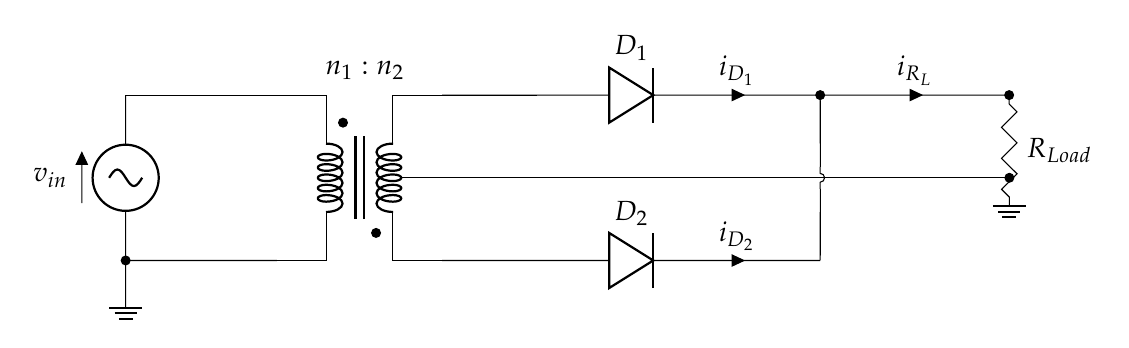
\begin{tikzpicture}[circuit ee IEC,scale=1.2]
		\begin{scope}[set resistor graphic=var resistor IEC graphic]
			\def\x{4}
			\draw (0,0)  node[transformer core,circuitikz/inductors/coils=6](T){} (T.base) node[above, xshift=2pt, yshift=2pt]{$n_{1}:n_{2}$}
			(T.inner dot A1) node[circ]{}
			(T.inner dot B2) node[circ]{} ;
			\draw (T.A2) to [short,-*] ($(T.A2)+(-0.4*\x,0)$)
			to [short] ($(T.A2)+(-0.4*\x,-0.50)$)
			node[tlground]{};
			\draw ($(T.A2)+(-0.4*\x,0)$) to [sV={$v_{in}$}] ($(T.A1)+(-0.4*\x,0)$);
			\draw (T.A1) --++(-0.4*\x,0);
			\draw (T.B1) --++(1,0);
			\draw (T.B1) to [Do=$D_{1}$,i=$i_{D_{1}}$] ++(\x,0)
			to [crossing]($(T.B2)+(\x,0)$);
			\draw (T-L2.midtap) to [short] ++(1.11*\x,0) 
			to [short,-*] ++(0.5*\x,0);
			\draw (T.B2) to [Do={$D_{2}$},i=$i_{D_{2}}$,name=d2] ++(\x,0);
			\draw ($(T.B1)+(\x,0)$) to [short,*-*,i=$i_{R_{L}}$] ($(T.B1)+(1.5*\x,0)$) 
			to [resistor={info=$R_{Load}$}] ($(T-L2.midtap)+(1.61*\x,-0.3)$)  node[tlground]{}; 
			%\draw ($(T.B1)+(1.5*\x,0)$) to [resistor]  ++($(T-L2.midtap)+(1.5*\x,0)$);
			%\draw[dashed, {Triangle[round,open]}-] ($(T.B2)+(0.4,+0.3)$) -- ++(0,1.3) ;
			%\draw[-{Triangle[round,open]}] ($(T.B2)+(0,+0.3)$) -- ++(0,1.3);
		\end{scope} 
	\end{tikzpicture}
	\caption{Full-wave rectifier}
	\label{fig:rectifier}
\end{figure}

The Figure \ref{fig:rectifier} is the circuit of a full wave rectifier with 2 diodes where:

\begin{align*}
	V_{DC}&=\dfrac{2V_{max}}{\pi}=0.637V_{max}=0.7071V_{max}
\end{align*}




\end{document}
